
\chapter{20200322}
今回話したいこと
\begin{itemize}
    \item モチベーション
    \item 層の定義とB-sheafの定義.
    \item 環つき空間と$O_X$-modの層
    \item アフィンスキームの層(イメージ)
    \item $M$加群から準連接層の構成
    \item 準連接層の定義と性質
    \item アフィンスキーム上の準連接層と加群の誘導する層の関係
    \item 連接層の定義と性質
    \item アフィンスキームの場合の準連接層のコホモロジー
    \item 射影スキームの構成
    \item 射影スキームによるtwist
    \item 射影スキーム上の準連接層,連接層の特徴づけ
    \item 射影スキーム上の連接層のコホモロジーの計算
\end{itemize}

\subsection{モチベーション}
このセミナーではしばらく周期の話をする。
\begin{itemize}
\item $X$: $\overline{\mathbb{Q}}$上の代数多様体
\item $Z \subset X$: closed subvariety
\item $\gamma \in H_n(X^{an}, Z^{an}, \mathbb{Z})$:相対特異ホモロジー類
\item $\omega \in H_{dR}^n(X, \mathbb{Z})$をde Rhamコホモロジー類
\end{itemize}
この時$[X, Z, n ,\gamma, \omega]$を抽象的周期という.
前回のセミナーにて代数的なドラムの定理を示した。
改めて定理を記述すると
$X$を$\mathbb{C}$上の射影代数多様体とした時,
\begin{equation*}
  H^q(X_an, \mathbb{C}) = \mathcal{H}^q(X, \Omega_{alg})
\end{equation*}
となる.

前回はこれを二重複体の理論を使って証明した.
ただし,解析と代数との直接の関係はSerreのGAGAを用いて使った.
そこで今回次回の二回はSerreのGAGAを目標とする.
GAGAは射影代数多様の連接層とその複素化が作る連接層に対応があることを示すが。
連接層の一般論自体はそれ以前の論文で行われている。
またGAGA自体がスキーム論以前なので、スキーム論的にまとめ直したい.

ということで今回は準連接層や連接層を構成し,特に射影スキーム上の連接層のコホモロジーを計算したい。

\subsection{Preliiminary}

\subsection{global sectionで生成される層と準連接層}

\begin{screen}
\begin{dfn}
  
\end{dfn}
\end{screen}


大域切断で生成される層
準連接層の定義
$A$加群$M$が作る層
準連接層の操作に対する性質
アフィンスキーム上の準連接層の性質
連接層の定義と性質
ネーター環上のアフィンスキームの場合の連接層と加群の関係
Principal Open setを使ったチェックコホモロジーの計算
射影スキームの定義と基本的な性質
射影空間の性質
射影スキーム上の準連接層と連接層の構成
射影スキームの場合の次数つき加群と連接層の関係
(Remarkするだけ上野 定理5.21)
射影空間の連接層のコホモロジーの計算

\section{Coherent sheaves on scheme}
\subsection{sheaves of modules}

\begin{screen}
\begin{dfn}
 $(X, O_X)$をringed spaceとする.$X$上のアーベル群の層$\mathcal{F}$が$O_X$-加群であるとは,
 \begin{itemize}
   \item $X$の任意のopen set $U$に対し,$F(U)$は$O_X(U)$加群となる.
   \item $V \subset U$に対し,以下となる.

   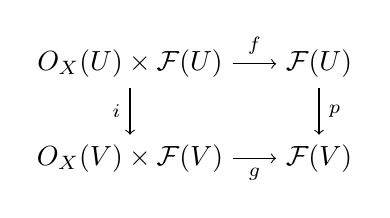
\begin{tikzpicture}[auto]
   \node (a) at (0, 1.2) {$O_X(U) \times \mathcal{F}(U)$};
   \node (x) at (2.4, 1.2) {$\mathcal{F}(U)$};
   \node (b) at (0, 0) {$O_X(V) \times \mathcal{F}(V)$};
   \node (y) at (2.4, 0) {$\mathcal{F}(V)$};
   \draw[->] (a) to node {$\scriptstyle f$} (x);
   \draw[->] (x) to node {$\scriptstyle p$} (y);
   \draw[->] (a) to node[swap] {$\scriptstyle i$} (b);
   \draw[->] (b) to node[swap] {$\scriptstyle g$} (y);
   \end{tikzpicture}
\end{itemize}
\end{dfn}
\end{screen}


この時,$\mathcal{F},\mathcal{G}$のテンソル積,$\mathcal{F} \otimes_{O_X} \mathcal{G}$を
\begin{equation*}
U \mapsto \mathcal{F}(U) \otimes_{O_X(U)} \mathcal{G}(U)
\end{equation*}
の層化したものを$\mathcal{F} \otimes_{O_X} \mathcal{G}$で表す.
また$(\mathcal{F} \otimes_{O_X} \mathcal{G})_x = \mathcal{F}_x \otimes_{O_X, x} \mathcal{G}_x$となる.
これは\ref{tensor module}で示す.


\begin{screen}
\begin{dfn}
$(X, O_X)$加群$\mathcal{F}$に対し,$\mathcal{F}$が$x \in X$でglobal sectionで生成されるとは,
\begin{equation*}
  O_{X,x} \otimes \mathcal{F}(X) \twoheadrightarrow \mathcal{F}_x
\end{equation*}
となること.
$\forall x \in X$でglobal sectionで生成される時,$\mathcal{F}$はglobal sectionで生成されるという.
$S \subset \mathcal{F}(X)$に対し,$\{s_x \mid s \in S\}$が$\mathcal{F}_x$を生成する時$S$で生成されるという.
\end{dfn}
\end{screen}

\begin{lem}
 $\mathcal{F}$がglobal sectionで生成されていることと$O_X^{(I)} \twoheadrightarrow \mathcal{F}$と同値.
\end{lem}
\begin{proof}
$O_X^{(I)} \twoheadrightarrow \mathcal{F}$ならば$\mathcal{F}$がglobal sectionで生成されていることを示す.

   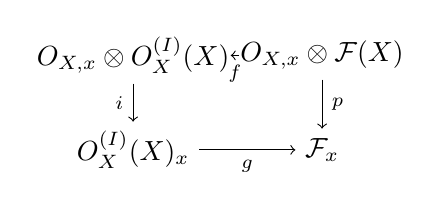
\begin{tikzpicture}[auto]
   \node (a) at (0, 1.2) {$O_{X,x} \otimes O_X^{(I)}(X) $};
   \node (x) at (2.4, 1.2) {$O_{X,x} \otimes \mathcal{F}(X)$};
   \node (b) at (0, 0) {$O_X^{(I)}(X)_x$};
   \node (y) at (2.4, 0) {$\mathcal{F}_x $};
   \draw[->] (a) to node {$\scriptstyle f$} (x);
   \draw[->] (x) to node {$\scriptstyle p$} (y);
   \draw[->] (a) to node[swap] {$\scriptstyle i$} (b);
   \draw[->] (b) to node[swap] {$\scriptstyle g$} (y);
   \end{tikzpicture}

が成り立ち,$i$は$O_X^{(I)}$は$O_X$加群としてglobal sectionで生成されているので全射.
また,$g$は仮定から全射となる.よって$p$は全射となるので,global sectionで生成されている.

逆を示す.$S$として$\mathcal{F}(X)$を取ることにより,必ず$\mathcal{F}$を生成する$S$が存在する.
また,$e_s \in O_X^S(U)$を$e_s(s) = 1, e_s(t) = 0$となる元とし,
$O_X^{S}(U) \to \mathcal{F}(U), \sum_{s \in S} a_s e_s \mapsto a_s s_U$とすれば,
これは層の間の射となり,全射性も言える.
\end{proof}


\begin{screen}
\begin{dfn}
$(X, O_X)$加群の層$\mathcal{F}$が\textbf{quasi coherent shaef}とは$\forall x \in X$に対し,$x \in U$が存在し,
\begin{equation*}
  O_X^{(J)}|_U \to O_X^{(I)}|_U \to \mathcal{F}|_U
\end{equation*}
がexactとなることを言う.
\end{dfn}
\end{screen}

\subsection{Quasi-Coherent Sheaves on an affine scheme}
$X = \mathrm{Spec}A$の時にquasi-coherent sheafを構成する.
$M$を$A$-modする.
$\tilde{M}$という$O_x$-加群を構成する.
\begin{equation*}
\tilde{M}(D(f)) := M_f = M \otimes_A A_f
\end{equation*}
とする.
$D(g) \subset D(f)$の時,$V(g) \supset V(f)$なので,
$\cup_{f \in p}p  = \sqrt{(f)} \ni g$となる.よって$g^n = fb$とかける.これより

\begin{alignat*}{2}
 A_f & \to &  \ A_g \\
 \frac{a}{f^m} & \mapsto & \ \frac{b^ma}{g^{mn}}
\end{alignat*}

が定まり,それの誘導する射

\begin{alignat*}{2}
 M_f & \to &  \ M_g \\
 \frac{x}{f^m} & \mapsto & \ \frac{b^m x}{g^{mn}}
\end{alignat*}

が定義される.
この時$\{D(f)\}$上で$\tilde{M}$が$\mathcal{B}$-sheafになることを示す.
\begin{align*}
  & X = \cup D(f_i) \\
\Leftrightarrow & X = D \left(\sum (f_i) \right) \\
\Leftrightarrow & V \left(\sum (f_i) \right) = \emptyset
\end{align*}
この時,$\sum f_i = (1)$より,$\sum a_i f_i = 1$とかける.
よって$a_i$が$0$でない$f_i$を使い,$X = \cup_{i=1}^n D(f_i)$とかける.

$X$のfinite open coveringについて,$X$について層の定義を満たすことを示せば十分である.
$X$についての条件を満たせれば,$X=D(f)$の時について示せる,それは$D(f) \cup D(f_i)$がAffineになるので,$D(f)$というスキームのfinte open coveringについて示せる.
また,finite open coverの時に言えれば,compactなのでopen coverに対し,affin finte open coverが取れ、そこ上で成り立つことを示せばよい。
特に
\subsection{Coherent sheaves}


\begin{lem}
\label{tensor module}
$X$上の$O_X$加群$\mathcal{F},\mathcal{G}$のテンソル積,$\mathcal{F} \otimes_{O_X} \mathcal{G}$を
$\mathcal{F} \otimes_{O_X} \mathcal{G}(U) := \mathcal{F}(U) \otimes_{O_X(U)} \mathcal{G}(U)$とすると層になる
また$(\mathcal{F} \otimes_{O_X} \mathcal{G})_x = \mathcal{F}_x \otimes_{O_X, x} \mathcal{G}_x$となる.
\end{lem}
環つき空間をスキームの場合に限定して示す. 局所的なので、$X$をアフィンスキームと思って良い.

\begin{lem}
$S^{-1}N \otimes M \sim S^{-1}(N \otimes M)$
\end{lem}
真面目に元をおえば示せる.


\begin{lem}
$S^{-1}(N \otimes M) \sim S^{-1}N \otimes_{S^{-1}R} S^{-1}M$
\end{lem}
これは$S^{-1}N = N \otimes S^{-1}R$より
\begin{equation*}
  S^{-1}N \otimes_{S^{-1}R} S^{-1}M \sim N \otimes S^{-1}R \otimes_{S^{-1}R} S^{-1}M \sim N \otimes S^{-1}M \sim  S^{-1}(N \otimes M)
\end{equation*}
となる.

これを使うことにより,スキームに対しては成り立つことがわかる.
おそらく,一般の場合は上と近い形で
$O(V) \otimes_{O(U)} M(U) \otimes N(V) \to M(V) \otimes N(V)$と
$N(U) \otimes M(U) \to O(V) \otimes N(U) \otimes M(V)$とを使いながら,これのらindcutive limitが一致することを示せばよいはず。


\section{Projective Scheme}

Projcetive Schemeの定義をする.
GAGAの対象となる射影代数多様体は$\mathbb{P}^n_{\mathbb{C}}$のclosed subschemeである.

\begin{dfn}
$B$が次数つき$A$代数であるとは
$B = \oplus B_n$とかけ,$B_n B_m \subset B_{n+m}$となること
\end{dfn}



\begin{lem}
  $f \in B_+$をdegree $r$のhomogeneousな元とする.
\begin{enumerate}
  \item canonicalな射は$\theta: D_+(f) \to \mathrm{Spec}B_{(f)}$同相となる
  \item $D_+(g) \subset D_+(f)$の時,$\alpha = g^r f^{- \mathrm{deg} g}$とする.
  この時$\theta(D_+(g)) = D(\alpha)$
  \item 自然な射$B_{(f)} \to B_{(g)}$は$(B_{(f)})_{\alpha} = B_{(g)}$をinduceする.
  \item その他いろいろ
\end{enumerate}
\end{lem}
1を示す.
方針は以下の通り.
\begin{itemize}
  \item $\mathrm{Proj}B$が$\mathrm{Spec}B$の部分位相であることを示す.
  \item 環の間の射を用いて自然な射を誘導し,連続であることを示す
  \item 射が全射であることを示す
  \item 射が単射であることを示す.
  \item 開写像であることを示す.
\end{itemize}

\begin{screen}
\begin{dfn}
  $X_i:=\mathrm{Spec}A[T_iT_j^{-1}]$とすると$X_{ij} = X_{ji}$となるので,これを張り合わせたものを$A$のProjective Spaceといい$\mathbb{P^n}_A$で表す.
  Projective Spaceのclosed subschemeをProjective Schemeという.
\end{dfn}
\end{screen}
